%FIXME:
%	nepouziva se NFSS
%	tilda
\documentclass[10pt,a4paper,notitlepage]{article}

\usepackage[left=1.5cm,text={18cm, 25cm},top=2.5cm]{geometry}
\usepackage{color}
\usepackage[czech]{babel}
%\usepackage[IL2]{fontenc}
\usepackage[T1]{fontenc}
\usepackage[utf8]{inputenc}
\usepackage{listings}
\usepackage{graphicx}

\newcommand{\myUrl}[1]{{\color{blue}{#1}}}
\newcommand{\myuv}[1]{\quotedblbase #1\textquotedblleft}
\newcommand{\tab}[1]{\hspace{.2\textwidth}\rlap{#1}}
\newcommand{\bigO}{\ensuremath{\mathcal{O}}}%

\author{Michal Šrubař\\xsruba03@stud.fit.vutbr.cz}
% date s prazdnym argumentem zpusobi neuvedeni date v titulku
\date{\today}	
\title{PDS: Firewall}



\begin{document}

\maketitle

\section{Úvod} \label{sec:hladka_sazba}
Tato dokumentace popisuje způsob řešení a algoritmus, který byl použit při
implementaci linuxového firewallu pro předmět
PDS\footnote{\myUrl{http://www.fit.vutbr.cz/study/course-l.php.cs?id=6391}}. Zadáním
bylo implementovat modul pro linuxové jádro, využívající
netfilter\footnote{\myUrl{http://www.netfilter.org/}}, a uživatelksou aplikaci pro
komunikaci s~tímto modulem. Řešení tohoto projektu bylo inspirováno online
návodem \textit{„How to Write a Linux Firewall in Less than 1000 Lines of
Code“}\cite{one},
který napsal Liu Feipeng. Kompletní text zadání je možné nalézt v~souboru
\texttt{doc/zadani.txt}.

\subsection{Popis řešení}
Firewall je rozdělen na dvě části a to modul pro linuxové jádro,
\textit{pdsfw.ko}, a klientskou aplikaci \textit{pdscli}. 

\subsection{2.3 Syntaktická kontrola pravidel}
Pravidla musí mít následující formát: 
\\
\\
\texttt{<number> <action> <protocol> from <src IP> to <dest IP> [src-port <srcPort>] [dst-port <dstPort>]}, 
\\
\\
kde jednotlivé složky mají následující význam:

\begin{table}[ht]
\begin{left}	
\begin{tabular}{ l  l }
  - \texttt{<number>}: & číslo pravidla, \\ 
  - \texttt{<action>}: & allow | deny, \\
  - \texttt{<protocol>}: & tcp | udp | icmp | ip, \\
  - \texttt{<src IP>}: & IPv4 adresa | any, \\
  - \texttt{<dst IP>}: & IPv4 adresa | any, \\
  - \texttt{<srcPort>}: & číslo portu, \\
  - \texttt{<dstPort>}: & číslo portu. \\
  \end{tabular}
  \end{center}
\end{table}
\\
Příklad pravidla:
\texttt{20 allow udp from any to 8.8.8.8 src-port 53}
\\
\\
Kontrola syntaxe pravidel, ať už specifikovaných v~souboru nebo pravidla
zadaného jako argument programu za přepínačem \texttt{-a}, se provádí pomocí nástrojů
\textit{flex}\footnote{\myUrl{http://flex.sourceforge.net/}} a
\textit{yacc}\footnote{\myUrl{http://dinosaur.compilertools.net/yacc/}}. Pomocí nástroje
flex je generován lexikální analyzátor, který čte jednotlivé lexikální jednotky
a předává je nástroji yacc, který poté provádí kontrolu syntaxe čtených pravidel
podle zvolené gramatiky. Tento proces popisuje obrázek \ref{pic:1}.

\begin{figure}[h]	% h means place the figure here
\centering % center
\scalebox{0.85}{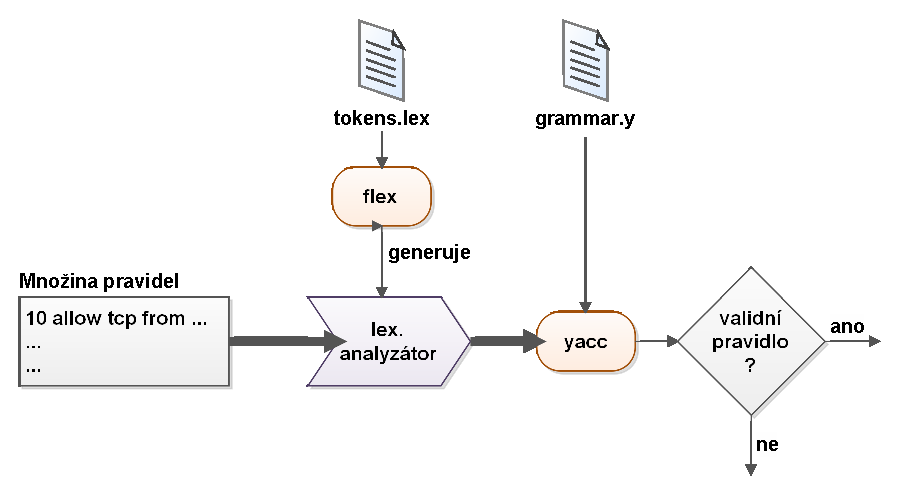
\includegraphics{imgs/rule_check.eps}}
\caption{Proces kontroly syntaxe pravidel.}
\label{pic:1}
\end{figure}

Definici lexikálních jednotek neboli tzv. \textit{lexémů}, které má lex.
analýzator rozpoznávat, se provádí pomocí regulárních výrazů. Pro rozpoznávání
jednotlivých lexémů byly zvoleny regulární výrazy, které specifikuje tabulka
\ref{regex}. Detailní informace viz. soubor \texttt{tokens.lex}. Význam
  jednotlivých vzorů je možné nálezt v~dokumentaci nástroje flex
  \footnote{\myUrl{http://flex.sourceforge.net/manual/Patterns.html\#Patterns}}.


\begin{table}[ht]
%zarovnani cele tabulky na stred dokumentu
\begin{left}	
\begin{tabular}{| l | l | l |} \hline
  \textbf{Řetězec} & \textbf{Vzor} & \textbf{Popis}\\ \hline
  <number> & \char"5E $$([1-9]|[0-9][0-9]|[0-9][0-9][0-9]|[0-9][0-9][0-9][0-9]|$$ & Rozsah hodnot ID pravidel\\ 
   & $$[0-9][0-9][0-9][0-9][0-9]|[0-9][0-9][0-9][0-9][0-9][0-9])$$ &  je omezen na interval (1,1000000).\\ \hline

  <action> & allow | deny | ALLOW | DENY & klíčová slova \\ \hline
  <protocol> & tcp | udp | icmp | ip | TCP | UDP | ICMP | IP &klíčová slova \\ \hline
  from & from | FROM & klíčová slova\\ 
  to & to | TO & \\ \hline

  <src IP> & $$(((\{DIGIT\}\{1,2\})|(1\{DIGIT\}\{2\})|(2[0-4]\{DIGIT\})|(25[0-5]))\.)$$ &
  Hodnoty validních IPv4 adres jsou \\
  <dest IP> & $$\{3\}((\{DIGIT\}\{1,2\})|(1\{DIGIT\}\{2\})|$$ &
  omezeny na rozsah 0.0.0.0 až \\
   & $$(2[0-4]\{DIGIT\})|(25[0-5]))|any|ANY$$ & 255.255.255.0. \\ \hline

  src-port & src-port|SRC-PORT & klíčová slova\\ 
  dst-port & dst-port|DST-PORT & \\ \hline
  
  <srcPort> & $$([0-9]{1,4}|[1-5][0-9]{4}|6[0-4][0-9]{3}$$ & Hodnoty přijatelných portů jsou \\
  <dstPort> & $$|65[0-4][0-9]{2}|655[0-2][0-9]|6553[0-5])$$ & omezeny na interval (0, 65535).\\ \hline

  \end{tabular}
  \caption{Použité regulární výrazy.}
  \label{regex}
  \end{center}
\end{table}

\newpage
\subsection{Gramatika}
Pro kontrolu syntaxe je použita bezkontextová gramatika \textit{G = (N, T, P,
S)}, kde:

\lstset{
  %basicstyle=\itshape,
  %basicstyle=\ttfamily,
  xleftmargin=3em,
  literate={->}{$\rightarrow$}{2}
           {α}{$\alpha$}{1}
           {δ}{$\delta$}{1}
}

\begin{lstlisting}
N = {rules, rule, port}
T = {<number>, <action>, <protocol>, from, <src IP>, to, <dest IP>, src-port, 
    <srcPort>, dst-port, <dstPort>}
P = {
  rules -> E | rule,
  rule -> <number> <action> <protocol> from <src IP> to <dest IP> port rules,
  port -> E | src-port <srcPort> | dst-port <dstPort> | 
          src-port <srcPort> dst-port <dstPort>
  }
S~= rules
\end{lstlisting}

Poznámka: Symbol E reprezentuje prázdný řetězec \epsilon.
\\

Jak je vidět z~pravidel gramatiky G, soubor pravidel může být buď prázdný, nebo
se skládát z~pravidel, která obsahují id, akci, protokol a zdrojovou a cílovou
IP adresu, případně může pravidlo specifikovat také cílový/zdrojový port. Zápis
gramatiky je možné nalézt v~souboru \texttt{grammar.y}.

\subsection{Vzájemná komunikace}
Komunikace mezi modulem pdsfw a klientskou aplikaci, kterou popisuje obrázek
\ref{pic:2}, se provádí prostřednictvím virtuální filesystému \texttt{/proc}.
Při zavedení modulu do jádra je vytvořen soubor \texttt{/proc/pdsfw\_xsruba03}.
Při každém pokusu o~čtení toho souboru je tato událost zachycena modulem a
zpracována. Zpracování se rozumí zapsaní pravidel firewallu z~datové struktury
do daného souboru. Zápis do toho souboru je taktéž událost, kterou modul
zpracovává. Vždy když chce klientská aplikce získat seznam aktuálně použivaných
pravidel nebo provést odstranění nekterého z~pravidel, pak zapíše do souboru
\texttt{/proc/pdsfw\_xsruba03} daný příkaz, který modul zpracuje a vyhodnotí.
Čtení aktuálně použivaných pravidel je na straně kernel modulu implementováno
pomocí sekvenčních souborů, které odstraňují limit velikosti
stránky\footnote{makro PAGE\_SIZE}, který by zabraňoval zápis pravidel, jejichž
délka v~textové podobě, by překročila velikost stránky, což je typicky 4096B.

\begin{figure}[h]	% h means place the figure here
\centering % center
\scalebox{0.85}{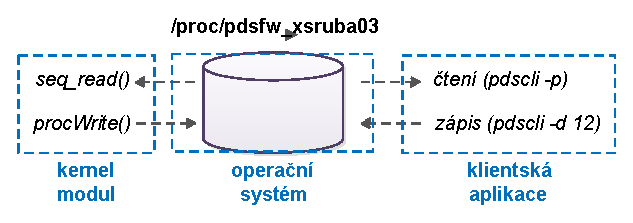
\includegraphics{imgs/proc_communication.eps}}
\caption{Komunikace mezi kernel modulem a klientskou aplikací.}
\label{pic:2}
\end{figure}

\subsection{Datové struktury a klasifikace paketů}
Pro uložení pravidel je použit linuxový obousměrně vázaný seznam nad kterým je
definována relace uspořádání nad množinou čísel pravidel. Tato relace je
zachována i při vkládání nových pravidel.

Pravidla se skládají ze čtyř dimenzí, které jsou protokol, zdrojová IP adresa,
cílová IPv4 adresa, zdrojový port a cílový port. Každý příchozí/odchozí paket je
porovnám s~každým pravidlem a to s~každou jeho dimenzí, dokud není nalezena
shoda\footnote{first-match policy}, jestliže se všechny
dimenze schodují, pak byla nalezena shoda pro dané pravidlo a je aplikovaná
příslušná akce, tj. zahození/propuštění daného paketu. Jestliže paket nesplňuje
podmínku shody všech dimenzí žádného pravidla, pak je propuštěn. Jednotlivé
dimenze pravidel jsou porovnávány v~následujícím pořadí:

\begin{enumerate}
  \item protokol,
  \item zdrojová IPv4 adresa,
  \item cílová IPv4 adresa,
  \item zdrojový port,
  \item cílový port.
\end{enumerate}

Časová složitost vyhledávání v~takto zvolené datové struktuře samozdřejmě není
nejslepší. Označme \textit{l} jako počet pravidel v~seznamu a \textit{d} jako
počet porovnávaných hodnot každé položky, poté časová složitost vyhledávání bude
v~nejhorším případě \bigO \textit{(l*d)}, což se blíží kvadratické složitosti.
S~využitím lepší datových struktur a algoritmů jako je například stromové
vyhledávání\footnote{tries, grid of tries} by bylo možné dosáhnout složitosti
časové složitosti \bigO \textit{n*log(n)}.



%\section{Instalace}
%Pro přeložení projektu je přiložen potřebný Makefile. Pro překlad tedy stačí
%provést: \\
%\texttt{\$ make}
%\\
%Po úspěšném překladu vzninkou dva binární soubory:
%\begin{enumerate}
%  \item \texttt{pdsfw.ko}
%  \item \texttt{pdscli}
%\end{enumerate}
%
%\section{Příklad použití}
%Nejprve je potřeba zavést příslušný modul do jádra:
%\\
%\texttt{\$ insmod pdsfw.ko}
%\\
%
%Úspěšné zavedení modulu je možné ověřit ve výpisu souboru \texttt{/var/log/messages}
%TODO: pridat vystupy z~finalni aplikace
%
%Po úspěšném zavedení modulu je možné používat klientskou aplikaci \texttt{pdscli}.
%Nejprve přídáme do firewallu nějaká pravidla, která máme uložena v~souboru
%\texttt{test\_fwrules.in}.
%
%\texttt{./pdscli -f test\_fwrules.in}
%
\begin{thebibliography}{9}

\bibitem{one}
  Liu Feipeng
  \emph{How to Write a Linux Firewall in Less than 1000 Lines of Code Part 1–Overview},
  July 23, 2011,
  \myUrl{http://www.roman10.net/a-linux-firewall-using-netfilter-part-1overview/}

\end{thebibliography}

\end{document}
